\section{Literature Review}

\subsection{Stellar Model}

A stellar model is a mathematical model that describes a star structure and evolution. Stellar structure models describe the internal structure of a star in detail and make predictions about the luminosity, the color and the future evolution of the star. Different classes and ages of stars have different internal structures, reflecting their elemental makeup and energy transport mechanisms. Stellar evolution is the process by which a star changes over the course of its lifetime. A stellar evolutionary model is a mathematical model that can be used to compute the evolutionary phases of a star from its formation until it becomes a remnant.

Example of a stellar model is the Standard Solar Model (SSM) which is a mathematical model that describes the Sun as a spherical ball of gas, and it's used to test the validity of stellar evolution theory. The SSM is used to test the validity of stellar evolution theory. In fact, the only way to determine the two free parameters of the stellar evolution model, the helium abundance and the mixing length parameter (used to model convection in the Sun), are to adjust the SSM to fit the observed Sun.

\subsection{Neutrino}

An elementary particle first proposed by Pauli in 1931 and named by Fermi; the neutrino was to account for the missing energy released in $\beta$ decay. Due to conservation of electric charge, it must be neutral, and conservation of angular momentum requires it to have a spin of $\frac{1}{2}$. There are two types of neutrinos emitted in $\beta$ decay neutrino, e and antineutrino, e and they are emitted in $\beta$+ and $\beta$- decays respectively. The neutrino has a very small cross section, $\sigma$ of \SI{1.2e-43}{\centi\meter\squared} \shortcite{krane-1991}. Due to this, neutrinos can escape from the sun in about 2 seconds which is very fast compared to the 100,000 years for a photon \shortcite{rosso-2018}. The first neutrino was detected experimentally in the 1950s by Reines and Cowan using a nuclear reactor as the source where $\beta$- decays occur producing e.

\subsection{Neutrino Sources}
There are multiple sources of neutrino both on earth and extraterrestrial, for example the Cosmic Neutrino Background (CNB), Supernovae, Solar and Thermal neutrinos from the sun, Geoneutrinos and many more as shown in Figure~\ref{fig:Nsource} \shortcite{athar-2020}. 
\begin{figure}[H]
	\centering
	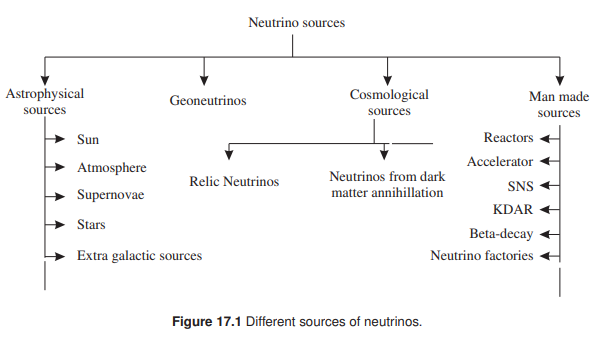
\includegraphics[width=\textwidth]{assets/NeutrinoSourcesSajjad.png}
	\caption{Neutrino sources.}
	\label{fig:Nsource}
\end{figure}

Most of them produce neutrinos through $\beta$ decays and electron(positron) capture like shown in Table~\ref{tab:reaction}  \shortcite{rosso-2018}:
\begin{table}[H]
	\centering
	\caption{Most common reaction that produce $\nu$.}
	\label{tab:reaction}
	\begin{tabular}{cc}
		\toprule
		Name & Reaction \\
		\midrule
		$\beta^+$ decays & $n\rightarrow p+e^-+\nu_e$ \\
		$\beta^-$ decays & $p\rightarrow n+e^++\bar\nu_e$ \\
		$e^-$ capture & $e^-+p\rightarrow n+\nu_e$ \\
		$e^+$ capture & $e^++n\rightarrow p+\bar\nu_e$ \\
		\bottomrule
	\end{tabular}
\end{table}
that produce $\nu$.

And unlike most other particles which are charged neutrinos can be assumed to come directly from their source as they are not deflected by magnetic field and unlike photons, neutrinos weakly interact making them able to pass through matter easily, the interaction length of a 1-TeV neutrino is about 2.5 million kilometers of water, or \SI{250}{\kilo\tonne\per\centi\meter\squared}, whereas high-energy photons are blocked by a few hundred \SI{}{\gram\per\centi\meter\squared} \shortcite{barenboim-2003}.

Graph 1 \shortcite{vitagliano-2020} shows the fluxes from different neutrino sources. The range of energy for different sources is quite huge, spanning over 24 orders of magnitude. 

\subsection{Solar Neutrino}
The sun through the thermonuclear fusion reaction produces a huge amount of e with energy the order of 1MeV. Since neutrino interaction with matter is weak, almost all the neutrino produced in the core goes out from the sun. The earth receives about \SI{6e10}{\centi\per\meter\squared\second} flux of solar neutrinos. For the sun 2.3\% of its nuclear energy production is in the form of MeV range electron neutrinos \shortcite{giunti-2007}. This comes from the effective nuclear reaction 
\begin{equation}
	4p+2e\rightarrow2{}^{4}He+2\nu{}_{e}+26.73MeV
\end{equation}
Which comes from several reaction chains and cycles \shortcite{vitagliano-2020}.

Table 2 \shortcite{vitagliano-2020} shows the different reactions that produce neutrinos that can be detected on earth that the sun produces in its thermonuclear process. While table 3 \shortcite{rosso-2018} shows the expectation of the solar neutrino flux from each branch coming to earth. Referring to table Graph 1, we can see the shape of the flux in a solid blue line labelled ``Solar (nuclear)''.

\subsection{Theoretical vs Experimental}

\subsubsection{Theoretical}
For the theoretical side of stellar physics, most of them are done in doing stellar modelling to predict structures and evolution of certain mass stars. Example of theoretical work done in neutrino is Stellar Neutrino Emission across the Mass–Metallicity Plane done by \shortcite{Farag_2020} where they explore neutrino emission from nonrotating, single-star models across six initial metallicities and 70 initial masses from the zero-age main sequence to the final fate. The data produced in the model are used in this research in order to train the model.

Since the time and computational power needed to run even one model is quite arduous, by using machine learning, the gap between the modelled grid can be predicted using machine learning.

\subsubsection{Experimental}
Due to neutrinos having an almost negligible mass and interact weakly with matter, the experiments that are required to detect them are usually done on a large scale in the range of km3 which can be setback by technological challenges \shortcite{ADDAZI2022103948}. Notable experiments include Super Kamiokande in Japan, the Sudbury Neutrino Observatory (SNO) in Canada, and the Jiangmen Underground Neutrino Observatory (JUNO) in China. Data from these experiments can validate the prediction obtained from a machine learning model.

\subsection{Current Works}



\subsection{Machine Learning}

Machine learning has been on the rise rapidly and can potentially revolutionize how we do sciences, including physics. According to \shortciteA{rodrigues-2023} even though machine learning can help solve fundamental problems in physics, many physicists still do not recognise the importance of these techniques. In physics, machine learning is often used in settings with complex problems and lots of data like in the large hadron collider (LHC) experiments where the data can reach up to ten of thousands of petabytes per year. 

Figure 2: Supervise machine learning pipeline
In Figure 2 \shortcite{rodrigues-2023}, usually in supervised learning 80\% of data is used to train the model while 20\% is for testing the model.
In research done by \shortcite{niu-2019}, by using Bayesian neural network (BNN) which is a machine learning technique, they manage to get results that well reproduce the experimental data with very high accuracy and provide reasonable uncertainty in half-life prediction as shown in Figure 3 compared to prediction done using calculation.  

Figure 3: $\beta$ decay half-life of Ni isotopes
Where the experimental values in NUBASE2016 are denoted by spheres. The half-life predictions with calculation are shown by the dotted line, and their counterparts improved by BNN-I2 and BNN-I4 approaches, and their uncertainties are shown by vertical line hatched region and green hatched region, respectively. The mean predicted half-lives of BNN-I4 approach are marked by the dashed line.
